\documentclass[12pt]{article}
\usepackage{tikz}
\usepackage{collcell}
\usepackage{xcolor}
\usepackage{pgf}

% Define the minimum and maximum values for gradient coloring
\newcommand*{\MinValue}{0}%
\newcommand*{\MaxValue}{1}%

% Apply gradient coloring based on the value
\newcommand{\ApplyGradient}[1]{%
    \pgfmathsetmacro{\PercentColor}{(#1-\MinValue)/(\MaxValue-\MinValue)*100}
    \hspace{-0.33em}\colorbox{blue!\PercentColor!white}{\textcolor{black}{#1}}
}

\newcolumntype{R}{>{\collectcell\ApplyGradient}c<{\endcollectcell}}
\renewcommand{\arraystretch}{0}
\setlength{\fboxsep}{3mm} % box size
\setlength{\tabcolsep}{0pt}

% PCA reconstructed Iothers Time Domain %

\begin{document}
\begin{table}[ht]
\centering
\caption{PCA reconstructed Iothers Time Domain}
\vspace{10pt} % Add more space here
\begin{tabular}{c *{5}{R}}
\multicolumn{1}{c}{} & \multicolumn{1}{c}{Matched} & \multicolumn{1}{c}{One-Head} & \multicolumn{1}{c}{One-Data} & \multicolumn{1}{c}{Random} & \multicolumn{1}{c}{Sensor} \\
Pearson's & 0.0000 & 0.0000 & 0.0000 & 0.0000 & 0.0470\\
\end{tabular}

% Color Scale
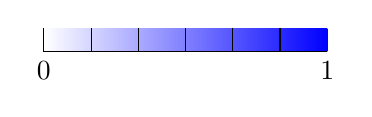
\begin{tikzpicture}[scale=0.6]
    \fill[left color=white, right color=blue] (0,0) rectangle (6,0.5);
    \draw (0,0) -- (6,0);
    \foreach \x in {0,20,...,100}
        \draw ({\x/20},0) -- ({\x/20},0.5);
    \node[below] at (0,0) {\MinValue};
    \node[below] at (6,0) {\MaxValue};
\end{tikzpicture}
\end{table}


% PCA reconstructed Iothers delta frequency %
\begin{table}[ht]
\centering
\caption{PCA reconstructed Iothers delta frequency}
\vspace{10pt} % Add more space here
\begin{tabular}{c *{5}{R}}
\multicolumn{1}{c}{} & \multicolumn{1}{c}{Matched} & \multicolumn{1}{c}{One-Head} & \multicolumn{1}{c}{One-Data} & \multicolumn{1}{c}{Random} & \multicolumn{1}{c}{Sensor} \\
AECno ort & 0.0000 & 0.0000 & 0.0000 & 0.0000 & 0.0780 \\
AECort & 0.0000 & 0.0000 & 0.0000 & 0.0000 & 0.0841 \\
ciPLV &  0.1069 & 0.1389 & 0.0253 & 0.1199 & 0.1441\\
\end{tabular}

% Color Scale
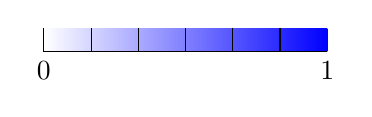
\begin{tikzpicture}[scale=0.6]
    \fill[left color=white, right color=blue] (0,0) rectangle (6,0.5);
    \draw (0,0) -- (6,0);
    \foreach \x in {0,20,...,100}
        \draw ({\x/20},0) -- ({\x/20},0.5);
    \node[below] at (0,0) {\MinValue};
    \node[below] at (6,0) {\MaxValue};
\end{tikzpicture}
\end{table}

% PCA reconstructed Iothers theta frequency %

\begin{table}[ht]
\centering
\caption{PCA reconstructed Iothers theta frequency}
\vspace{10pt} % Add more space here
\begin{tabular}{c *{5}{R}}
\multicolumn{1}{c}{} & \multicolumn{1}{c}{Matched} & \multicolumn{1}{c}{One-Head} & \multicolumn{1}{c}{One-Data} & \multicolumn{1}{c}{Random} & \multicolumn{1}{c}{Sensor} \\
AECno ort & 0.0000 & 0.0000 & 0.0000 & 0.0000 & 0.1272 \\
AECort & 0.0000 & 0.0000 & 0.0000 & 0.0000 & 0.0888 \\
ciPLV &  0.0891 & 0.1451 & 0.0605 & 0.1123 & 0.1276\\
\end{tabular}

% Color Scale
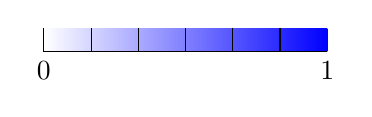
\begin{tikzpicture}[scale=0.6]
    \fill[left color=white, right color=blue] (0,0) rectangle (6,0.5);
    \draw (0,0) -- (6,0);
    \foreach \x in {0,20,...,100}
        \draw ({\x/20},0) -- ({\x/20},0.5);
    \node[below] at (0,0) {\MinValue};
    \node[below] at (6,0) {\MaxValue};
\end{tikzpicture}
\end{table}

% PCA reconstructed Iothers alpha frequency %

\begin{table}[ht]
\centering
\caption{PCA reconstructed Iothers alpha frequency}
\vspace{10pt} % Add more space here
\begin{tabular}{c *{5}{R}}
\multicolumn{1}{c}{} & \multicolumn{1}{c}{Matched} & \multicolumn{1}{c}{One-Head} & \multicolumn{1}{c}{One-Data} & \multicolumn{1}{c}{Random} & \multicolumn{1}{c}{Sensor} \\
AECno ort & 0.0000 & 0.0000 & 0.0000 & 0.0000 & 0.1985  \\
AECort & 0.0000 & 0.0000 & 0.0000 & 0.0000 & 0.1611 \\
ciPLV & 0.0898 & 0.1510 & 0.0421 & 0.0758 & 0.1362\\
\end{tabular}

% Color Scale
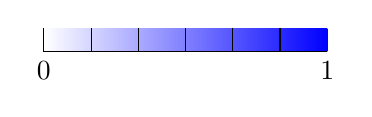
\begin{tikzpicture}[scale=0.6]
    \fill[left color=white, right color=blue] (0,0) rectangle (6,0.5);
    \draw (0,0) -- (6,0);
    \foreach \x in {0,20,...,100}
        \draw ({\x/20},0) -- ({\x/20},0.5);
    \node[below] at (0,0) {\MinValue};
    \node[below] at (6,0) {\MaxValue};
\end{tikzpicture}
\end{table}


% PCA reconstructed Iothers beta frequency %

\begin{table}[ht]
\centering
\caption{PCA reconstructed Iothers beta frequency}
\vspace{10pt} % Add more space here
\begin{tabular}{c *{5}{R}}
\multicolumn{1}{c}{} & \multicolumn{1}{c}{Matched} & \multicolumn{1}{c}{One-Head} & \multicolumn{1}{c}{One-Data} & \multicolumn{1}{c}{Random} & \multicolumn{1}{c}{Sensor} \\
AECno ort & 0.0000 & 0.0000 & 0.0000 & 0.0000 & 0.1951 \\
AECort & 0.0000 & 0.0000 & 0.0000 & 0.0000 & 0.1738\\
ciPLV &  0.0925 & 0.1551 & 0.0591 & 0.1001 & 0.1628\\
\end{tabular}

% Color Scale
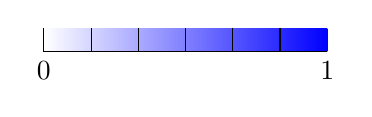
\begin{tikzpicture}[scale=0.6]
    \fill[left color=white, right color=blue] (0,0) rectangle (6,0.5);
    \draw (0,0) -- (6,0);
    \foreach \x in {0,20,...,100}
        \draw ({\x/20},0) -- ({\x/20},0.5);
    \node[below] at (0,0) {\MinValue};
    \node[below] at (6,0) {\MaxValue};
\end{tikzpicture}
\end{table}


% PCA reconstructed Iothers gamma frequency %

\begin{table}[ht]
\centering
\caption{PCA reconstructed Iothers gamma frequency}
\vspace{10pt} % Add more space here
\begin{tabular}{c *{5}{R}}
\multicolumn{1}{c}{} & \multicolumn{1}{c}{Matched} & \multicolumn{1}{c}{One-Head} & \multicolumn{1}{c}{One-Data} & \multicolumn{1}{c}{Random} & \multicolumn{1}{c}{Sensor} \\
AECno ort & 0.0000 & 0.0000 & 0.0000 & 0.0000 & 0.1620\\
AECort & 0.0000 & 0.0000 & 0.0000 & 0.0000 &  0.1837\\
ciPLV &  0.0815 & 0.1441 & 0.0379 & 0.1235 & 0.1611\\
\end{tabular}

% Color Scale
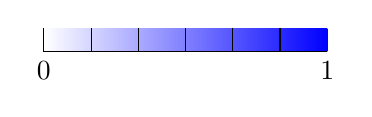
\begin{tikzpicture}[scale=0.6]
    \fill[left color=white, right color=blue] (0,0) rectangle (6,0.5);
    \draw (0,0) -- (6,0);
    \foreach \x in {0,20,...,100}
        \draw ({\x/20},0) -- ({\x/20},0.5);
    \node[below] at (0,0) {\MinValue};
    \node[below] at (6,0) {\MaxValue};
\end{tikzpicture}
\end{table}

% NON PCA reconstructed Iothers Time Domain %

\begin{table}[ht]
\centering
\caption{NON PCA reconstructed Iothers Time Domain}
\vspace{10pt} % Add more space here
\begin{tabular}{c *{5}{R}}
\multicolumn{1}{c}{} & \multicolumn{1}{c}{Matched} & \multicolumn{1}{c}{One-Head} & \multicolumn{1}{c}{One-Data} & \multicolumn{1}{c}{Random} & \multicolumn{1}{c}{Sensor} \\
Pearson's & 0.2104 & 0.6031 & 0.3554 & 0.2171 & 0.4631\\
\end{tabular}

% Color Scale
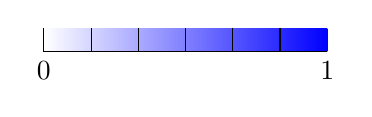
\begin{tikzpicture}[scale=0.6]
    \fill[left color=white, right color=blue] (0,0) rectangle (6,0.5);
    \draw (0,0) -- (6,0);
    \foreach \x in {0,20,...,100}
        \draw ({\x/20},0) -- ({\x/20},0.5);
    \node[below] at (0,0) {\MinValue};
    \node[below] at (6,0) {\MaxValue};
\end{tikzpicture}
\end{table}

% NON PCA reconstructed Iothers delta frequency %


\begin{table}[ht]
\centering
\caption{NON PCA reconstructed Iothers delta frequency}
\vspace{10pt} % Add more space here
\begin{tabular}{c *{5}{R}}
\multicolumn{1}{c}{} & \multicolumn{1}{c}{Matched} & \multicolumn{1}{c}{One-Head} & \multicolumn{1}{c}{One-Data} & \multicolumn{1}{c}{Random} & \multicolumn{1}{c}{Sensor} \\
AECno ort & 0.3366 & 0.9139 & 0.3706 & 0.3356 & 0.4503\\
AECort &  0.2091 & 0.5872 &  0.1047 &  0.2103 & 0.2457\\
ciPLV &  0.7340 & 0.5655 & 0.8009 & 0.7355 & 0.3260\\
\end{tabular}

% Color Scale
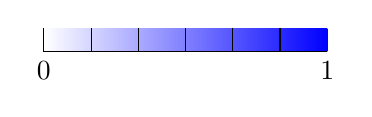
\begin{tikzpicture}[scale=0.6]
    \fill[left color=white, right color=blue] (0,0) rectangle (6,0.5);
    \draw (0,0) -- (6,0);
    \foreach \x in {0,20,...,100}
        \draw ({\x/20},0) -- ({\x/20},0.5);
    \node[below] at (0,0) {\MinValue};
    \node[below] at (6,0) {\MaxValue};
\end{tikzpicture}
\end{table}

% NON PCA reconstructed Iothers theta frequency %

\begin{table}[ht]
\centering
\caption{NON PCA reconstructed Iothers theta frequency}
\vspace{10pt} % Add more space here
\begin{tabular}{c *{5}{R}}
\multicolumn{1}{c}{} & \multicolumn{1}{c}{Matched} & \multicolumn{1}{c}{One-Head} & \multicolumn{1}{c}{One-Data} & \multicolumn{1}{c}{Random} & \multicolumn{1}{c}{Sensor} \\
AECno ort & 0.3432 & 0.9128 & 0.3650 & 0.3369 & 0.5361\\
AECort & 0.2211 & 0.6162 & 0.1817 & 0.2237 & 0.2919\\
ciPLV & 0.7261 & 0.5666 & 0.7875 & 0.7298 & 0.3393 \\
\end{tabular}

% Color Scale
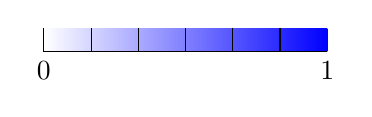
\begin{tikzpicture}[scale=0.6]
    \fill[left color=white, right color=blue] (0,0) rectangle (6,0.5);
    \draw (0,0) -- (6,0);
    \foreach \x in {0,20,...,100}
        \draw ({\x/20},0) -- ({\x/20},0.5);
    \node[below] at (0,0) {\MinValue};
    \node[below] at (6,0) {\MaxValue};
\end{tikzpicture}
\end{table}

% NON PCA reconstructed Iothers alpha frequency %

\begin{table}[ht]
\centering
\caption{NON PCA reconstructed Iothers alpha frequency}
\vspace{10pt} % Add more space here
\begin{tabular}{c *{5}{R}}
\multicolumn{1}{c}{} & \multicolumn{1}{c}{Matched} & \multicolumn{1}{c}{One-Head} & \multicolumn{1}{c}{One-Data} & \multicolumn{1}{c}{Random} & \multicolumn{1}{c}{Sensor} \\
AECno ort & 0.3452 & 0.9143 & 0.3698 & 0.3440 & 0.5749 \\
AECort &  0.2314 & 0.6335 & 0.1830 & 0.2294 & 0.3029\\
ciPLV & 0.7199 & 0.5525 & 0.8117 & 0.7316 & 0.3072\\
\end{tabular}

% Color Scale
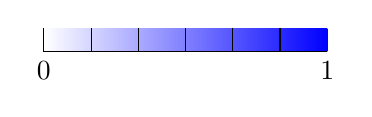
\begin{tikzpicture}[scale=0.6]
    \fill[left color=white, right color=blue] (0,0) rectangle (6,0.5);
    \draw (0,0) -- (6,0);
    \foreach \x in {0,20,...,100}
        \draw ({\x/20},0) -- ({\x/20},0.5);
    \node[below] at (0,0) {\MinValue};
    \node[below] at (6,0) {\MaxValue};
\end{tikzpicture}
\end{table}


% NON PCA reconstructed Iothers beta frequency %

\begin{table}[ht]
\centering
\caption{NON PCA reconstructed Iothers beta frequency}
\vspace{10pt} % Add more space here
\begin{tabular}{c *{5}{R}}
\multicolumn{1}{c}{} & \multicolumn{1}{c}{Matched} & \multicolumn{1}{c}{One-Head} & \multicolumn{1}{c}{One-Data} & \multicolumn{1}{c}{Random} & \multicolumn{1}{c}{Sensor} \\
AECno ort & 0.3560 & 0.9396 & 0.3623 & 0.3558 & 0.6254 \\
AECort & 0.2297 & 0.6676 & 0.1464 & 0.2282 & 0.4182\\
ciPLV & 0.7374 & 0.6033 & 0.8365 & 0.7443 & 0.4275\\
\end{tabular}

% Color Scale
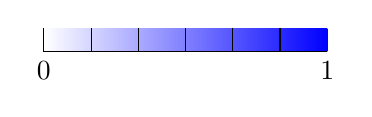
\begin{tikzpicture}[scale=0.6]
    \fill[left color=white, right color=blue] (0,0) rectangle (6,0.5);
    \draw (0,0) -- (6,0);
    \foreach \x in {0,20,...,100}
        \draw ({\x/20},0) -- ({\x/20},0.5);
    \node[below] at (0,0) {\MinValue};
    \node[below] at (6,0) {\MaxValue};
\end{tikzpicture}
\end{table}


% NON PCA reconstructed Iothers gamma frequency %

\begin{table}[ht]
\centering
\caption{NON PCA reconstructed Iothers gamma frequency}
\vspace{10pt} % Add more space here
\begin{tabular}{c *{5}{R}}
\multicolumn{1}{c}{} & \multicolumn{1}{c}{Matched} & \multicolumn{1}{c}{One-Head} & \multicolumn{1}{c}{One-Data} & \multicolumn{1}{c}{Random} & \multicolumn{1}{c}{Sensor} \\
AECno ort & 0.3418 & 0.9386 & 0.3680 & 0.3436 & 0.5773\\
AECort & 0.2142 & 0.6978 & 0.2328 & 0.2088 & 0.4259\\
ciPLV &  0.7410 & 0.6348 & 0.8220 & 0.7493 & 0.4573\\
\end{tabular}

% Color Scale
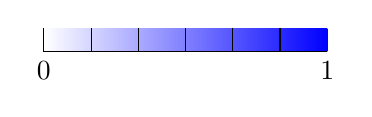
\begin{tikzpicture}[scale=0.6]
    \fill[left color=white, right color=blue] (0,0) rectangle (6,0.5);
    \draw (0,0) -- (6,0);
    \foreach \x in {0,20,...,100}
        \draw ({\x/20},0) -- ({\x/20},0.5);
    \node[below] at (0,0) {\MinValue};
    \node[below] at (6,0) {\MaxValue};
\end{tikzpicture}
\end{table}
\end{document}
